\documentclass[dvipdfmx, a4paper, 14Q, fleqn]{jreport}
\usepackage{../preamble/preamble_TeXManual}
\tcbuselibrary{breakable}
\begin{document}
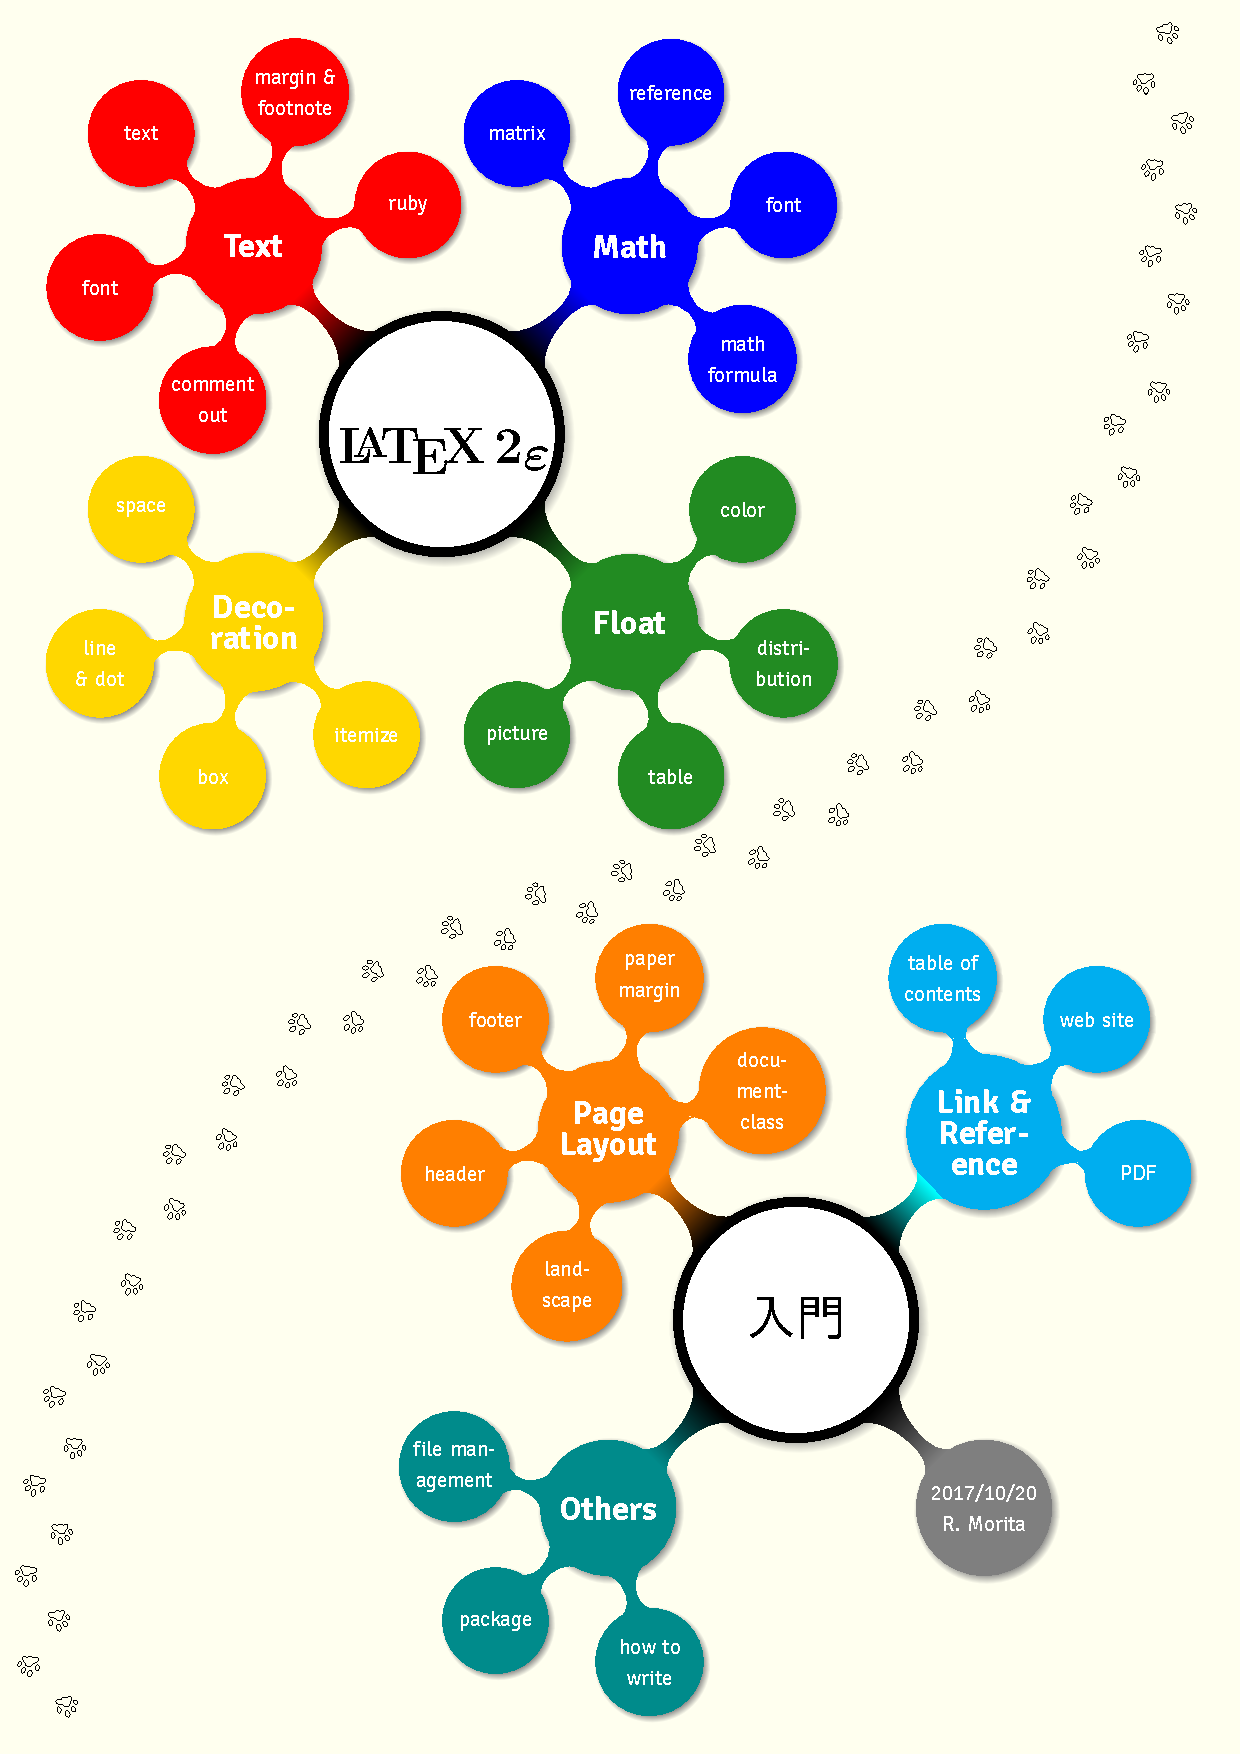
\includepdf[offset = 0mm -14mm]{../titlepage/titlepage_mindmap.pdf}
\subimport{../chapters/chapter0_introduction/}{introduction}
%\begin{tcolorbox}[breakable,enhanced jigsaw,title={Contents},fonttitle=\bfseries\Large,
  colback=yellow!10!white,colframe=red!50!black,before=\par\bigskip\noindent,
  interior style={fill overzoom image=goldshade.png,fill image opacity=0.25},
  colbacktitle=red!50!yellow!75!black,
  enlargepage flexible=\baselineskip,pad at break*=3mm,
  watermark color=yellow!75!red!25!white,
  watermark text={\bfseries\Large Contents},
  attach boxed title to top center={yshift=-0.25mm-\tcboxedtitleheight/2,yshifttext=2mm-\tcboxedtitleheight/2},
  boxed title style={enhanced,boxrule=0.5mm,
    frame code={ \path[tcb fill frame] ([xshift=-4mm]frame.west) -- (frame.north west)
    -- (frame.north east) -- ([xshift=4mm]frame.east)
    -- (frame.south east) -- (frame.south west) -- cycle; },
    interior code={ \path[tcb fill interior] ([xshift=-2mm]interior.west)
    -- (interior.north west) -- (interior.north east)
    -- ([xshift=2mm]interior.east) -- (interior.south east) -- (interior.south west)
    -- cycle;}  },
  drop fuzzy shadow]
\makeatletter
\@starttoc{toc}
\makeatother
\end{tcolorbox}

\begin{tcolorbox}[breakable,enhanced jigsaw,title={Contents},fonttitle=\bfseries\Large,
  colback=yellow!10!white,colframe=red!50!black,before=\par\bigskip\noindent,
  interior style={fill overzoom image=goldshade.png,fill image opacity=0.25},
  colbacktitle=red!50!yellow!75!black,
  enlargepage flexible=\baselineskip,pad at break*=3mm,
  watermark color=yellow!75!red!25!white,
  watermark text={\bfseries\Large Contents},
  attach boxed title to top center={yshift=-0.25mm-\tcboxedtitleheight/2,yshifttext=2mm-\tcboxedtitleheight/2},
  boxed title style={enhanced,boxrule=0.5mm,
    frame code={ \path[tcb fill frame] ([xshift=-4mm]frame.west) -- (frame.north west)
    -- (frame.north east) -- ([xshift=4mm]frame.east)
    -- (frame.south east) -- (frame.south west) -- cycle; },
    interior code={ \path[tcb fill interior] ([xshift=-2mm]interior.west)
    -- (interior.north west) -- (interior.north east)
    -- ([xshift=2mm]interior.east) -- (interior.south east) -- (interior.south west)
    -- cycle;}  },
  drop fuzzy shadow]
\makeatletter
\@starttoc{toc}
\makeatother
\end{tcolorbox}

\subimport{../chapters/chapter1_preparation/}{before_making_document}
\subimport{../chapters/chapter2_plane_text/}{how_to_write_plane_text}
\subimport{../chapters/chapter3_environment/}{about_environment}
\subimport{../chapters/chapter4_math/}{math_formula}
\subimport{../chapters/chapter5_pictures/}{about_pictures}
\subimport{../chapters/chapter6_tables/}{about_tables}
%\subimport{../chapters/chapterx7_macros/}{how_to_make_macros}			%未実装
\subimport{../chapters/chapter8_references_contents_links/}{references_contents_links}		%索引追加
\subimport{../chapters/chapterx_pagelayout/}{pagelayout}			%titlesec追加
\subimport{../chapters/chapterx_fonts/}{about_europian_fonts}	%書き足し予定(未定)
\subimport{../chapters/chapterx_fonts/}{about_japanese_fonts}	%書き足し予定(未定)
%\subimport{../chapters/chapterx_about_bibliography/}{how_to_write_bibliography} 	%未実装
\subimport{../chapters/chapterx_file_management/}{file_management}
\subimport{../chapters/chapterx_right_words/}{how_to_write_right_words}		%随時更新
\subimport{../chapters/chapterx_useful_packages/}{useful_packages} 			%随時更新
\subimport{../chapters/chapterx_others/}{other_topics}
\subimport{../bibliography/}{bibliography}
\end{document}

%physics・タイトルのデザインは書きたい

%以下実装未定
%mathabx, bbm, listing, 縦書き, textpos
%\subimport{../chapters/chapter_/}{TikZ}
%\subimport{../chapters/chapter_/}{tcolorbox}
%\subimport{../chapters/chapter_/}{スタイルファイルの作り方}
%\subimport{../chapters/chapter_/}{オンラインでTeXをする}
%\subimport{../chapters/chapter_/}{PythonTeX}